%%
%% licence       kaneton licence
%%
%% project       kaneton
%%
%% file          /home/mycure/kaneton/view/papers/kaneton/nomenclature.tex
%%
%% created       julien quintard   [tue mar  7 14:19:17 2006]
%% updated       julien quintard   [thu may  4 13:24:01 2006]
%%

%
% nomenclature
%

\chapter{Nomenclature}

In this chapter we will detail the kaneton nomenclature which is very
specific to the project.

Then, the reader will be able to understand the next chapters since the
kaneton documents heavily use the kaneton nomenclature.

Note that certain managers use another nomenclature for their own
purpose.

\newpage

%
% text
%

Like any other important project, the kaneton microkernel project
uses many terms to define very precise things.

The kaneton nomenclature was introduced to make communication between
developers easier. Indeed it is somethimes hard to speak widely using
terms like \textit{architecture-independent soure code},
\textit{architecture-dependent source code},
\textit{contiguous area of used physical memory},
\textit{contiguous area of free virtual memory}, etc..

The reader should notice that these terms are complex and a bit confused
when used together in the same sentence.

Then, kaneton people decided to introduce a well defined nomenclature
to make things clear.

We will so describe this nomenclature in the next sections.

%
% microkernel
%

\section{Microkernel}

The kaneton microkernel source code is composed of two majors parts, the
architecture-independent part and the architecture-dependent part.

The architecture-independent source code is called \textbf{core} and
make mainly reference to the kaneton managers. The architecture-dependent
source code is called \textbf{machdep} for \textit{machine-dependent}.

The kaneton microkernel is composed of \textbf{objects}. Technically,
an object, in kaneton terms, is simply a structure that begins with
a kaneton identifier. All kaneton objects are identifiers by kaneton
identifiers and are manipulated by kaneton capabilities.

An \textbf{identifier} is just a number referencing a kaneton object.
The kaneton microkernel reference implementation uses 64-bit identifiers.

A \textbf{capability} is a kind of cryptographic key used to reference
kaneton objects over the network.

Moreover, the kaneton microkernel is divided into subparts to make the
microkernel very clear to students. The subparts are called \textbf{managers}.

A \textbf{manager} is simply a piece of coherent code which takes care
of a unique kaneton object type. For example the \textit{segment manager}
provides simple operations to use physical memory.

The whole core is composed of managers which manage multiple kaneton objects.

A \textbf{segment} object describes a contiguous area of physical memory.
Each segment has a base address, a size, permissions and other properties.

A \textbf{region} object describes a contiguous area of virtual memory.
Each region references a segment meaning that a part of this segment
is mapped by this region.

An \textbf{as} or \textbf{address space} is an abstraction describing
a set of addressable memory addresses. An address space object is composed
of a set of segments listing the useable physical memory and a set of
regions listing the useable virtual memory.

A \textbf{thread} object is the kaneton active entity. Indeed, a thread
describes an execution context.

The \textbf{scheduler} manages threads using classes, behaviours and
priorities to compute the schedule priority.

A \textbf{task} object is an abstraction describing a complete execution
context with addressable memory and threads. A task is composed of
an address space and a set of threads. Note that kaneton tasks are
native multi-threaded tasks.

An \textbf{event} object describes an external event including hardware
events like interrupts as well as software events also known as system
calls.

The kaneton microkernel uses a very specific object called \textbf{set}.
A set object is an abstract data structure managed by the set manager.
A set is just used to store data without taking care of how it is technically
done. The set concepts was introduced to make the microkernel code as
clear as pseudo code.

We so might be able to easily represent the kaneton object hierarchy as
the following:

\begin{figure}[h]
  \begin{center}
    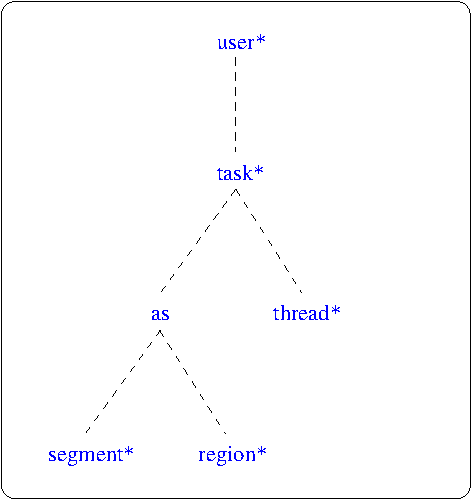
\includegraphics[scale=0.8]{figures/nomenclature_hierarchy.pdf}
    \caption{The kaneton object hierarchy.}
    \label{figure:nomenclature_hierarchy}
  \end{center}
\end{figure}

XXX est-ce que ce qui suit ne devrait pas etre mis dans coding-style ?

The kaneton core was implemented following a very strict source code
nomenclature we will now detail.

Each manager provides an interface to manipulate a kaneton object or
something else. The naming scheme used for these provided functions
is the explained below.

The function \textit{manager}\_\textbf{init}() initializes the whole
manager and the function \textit{manager}\_\textbf{clean}() cleans it.

The function \textit{manager}\_\textbf{show}() displays information
on a precise object while the function \textit{manager}\_\textbf{dump}()
displays information on every objects managed.

The function \textit{manager}\_\textbf{reserve}() reserves an object
given some properties and the function \textit{manager}\_\textbf{release}()
releases it.

The function \textit{manager}\_\textbf{clone}() clones an object. It is
important to understand that cloning an object does not just mean
generating an identical object. Indeed, cloning an object means creating
a new object with the same properties. Notice that the fact of creation
implies a new object so a new identifier.

The function \textit{manager}\_\textbf{give}() gives an object to another
entity.

The function \textit{manager}\_\textbf{flush}() cleans every objects
previously reserved depending on the implementation.

The \textit{manager} must be replaced by the manager name like \textit{as},
\textit{task}, \textit{segment} etc..

Moreover, the kaneton development environment are organized in a very
strict way to help students to find the files they are looking for. Indeed,
given a manager name \textit{manager}, the files in relation with this
manager are located in the directory listed below:

\begin{itemize}
  \item
    \textbf{kaneton/core/}\textit{manager}\textbf{/}\textit{manager}\textbf{.c}
  \item
    \textbf{kaneton/core/arch/}\textit{architecture}\textbf{/}\textit{manager}\textbf{.c}
  \item
    \textbf{kaneton/include/core/}\textit{manager}\textbf{.h}
  \item
    \textbf{kaneton/include/arch/}\textit{architecture}\textbf{/core/}\textit{manager}\textbf{.h}
\end{itemize}

%
% operating system
%

\section{Operating System}

The kaneton microkernel manages four different task classes.

A \textbf{program} is the lowest priviliged task f the system. The common
user programs are the well known UNIX{\copyright} binaries like
\textit{/bin/ls}, \textit{/bin/sh} etc..

A \textbf{service} is a microkernel server which provides a logical
service. For example, a service could be the \textit{Virtual File System}
which dispatches the calls to the filesystems to the correct servers.

A \textbf{driver} is a service which performs hardware communication.
For example, a \textit{Wireless driver} is a driver in the kaneton terms.

Finally, a \textbf{core} is a task which is a kind of super-driver in which
it has full rights on the whole machine.

A \textbf{module} is simply an additional file passed at the boot time.
